\begin{figure}
	\centering
	\begin{subfigure}{0.48\linewidth}
		\centering
		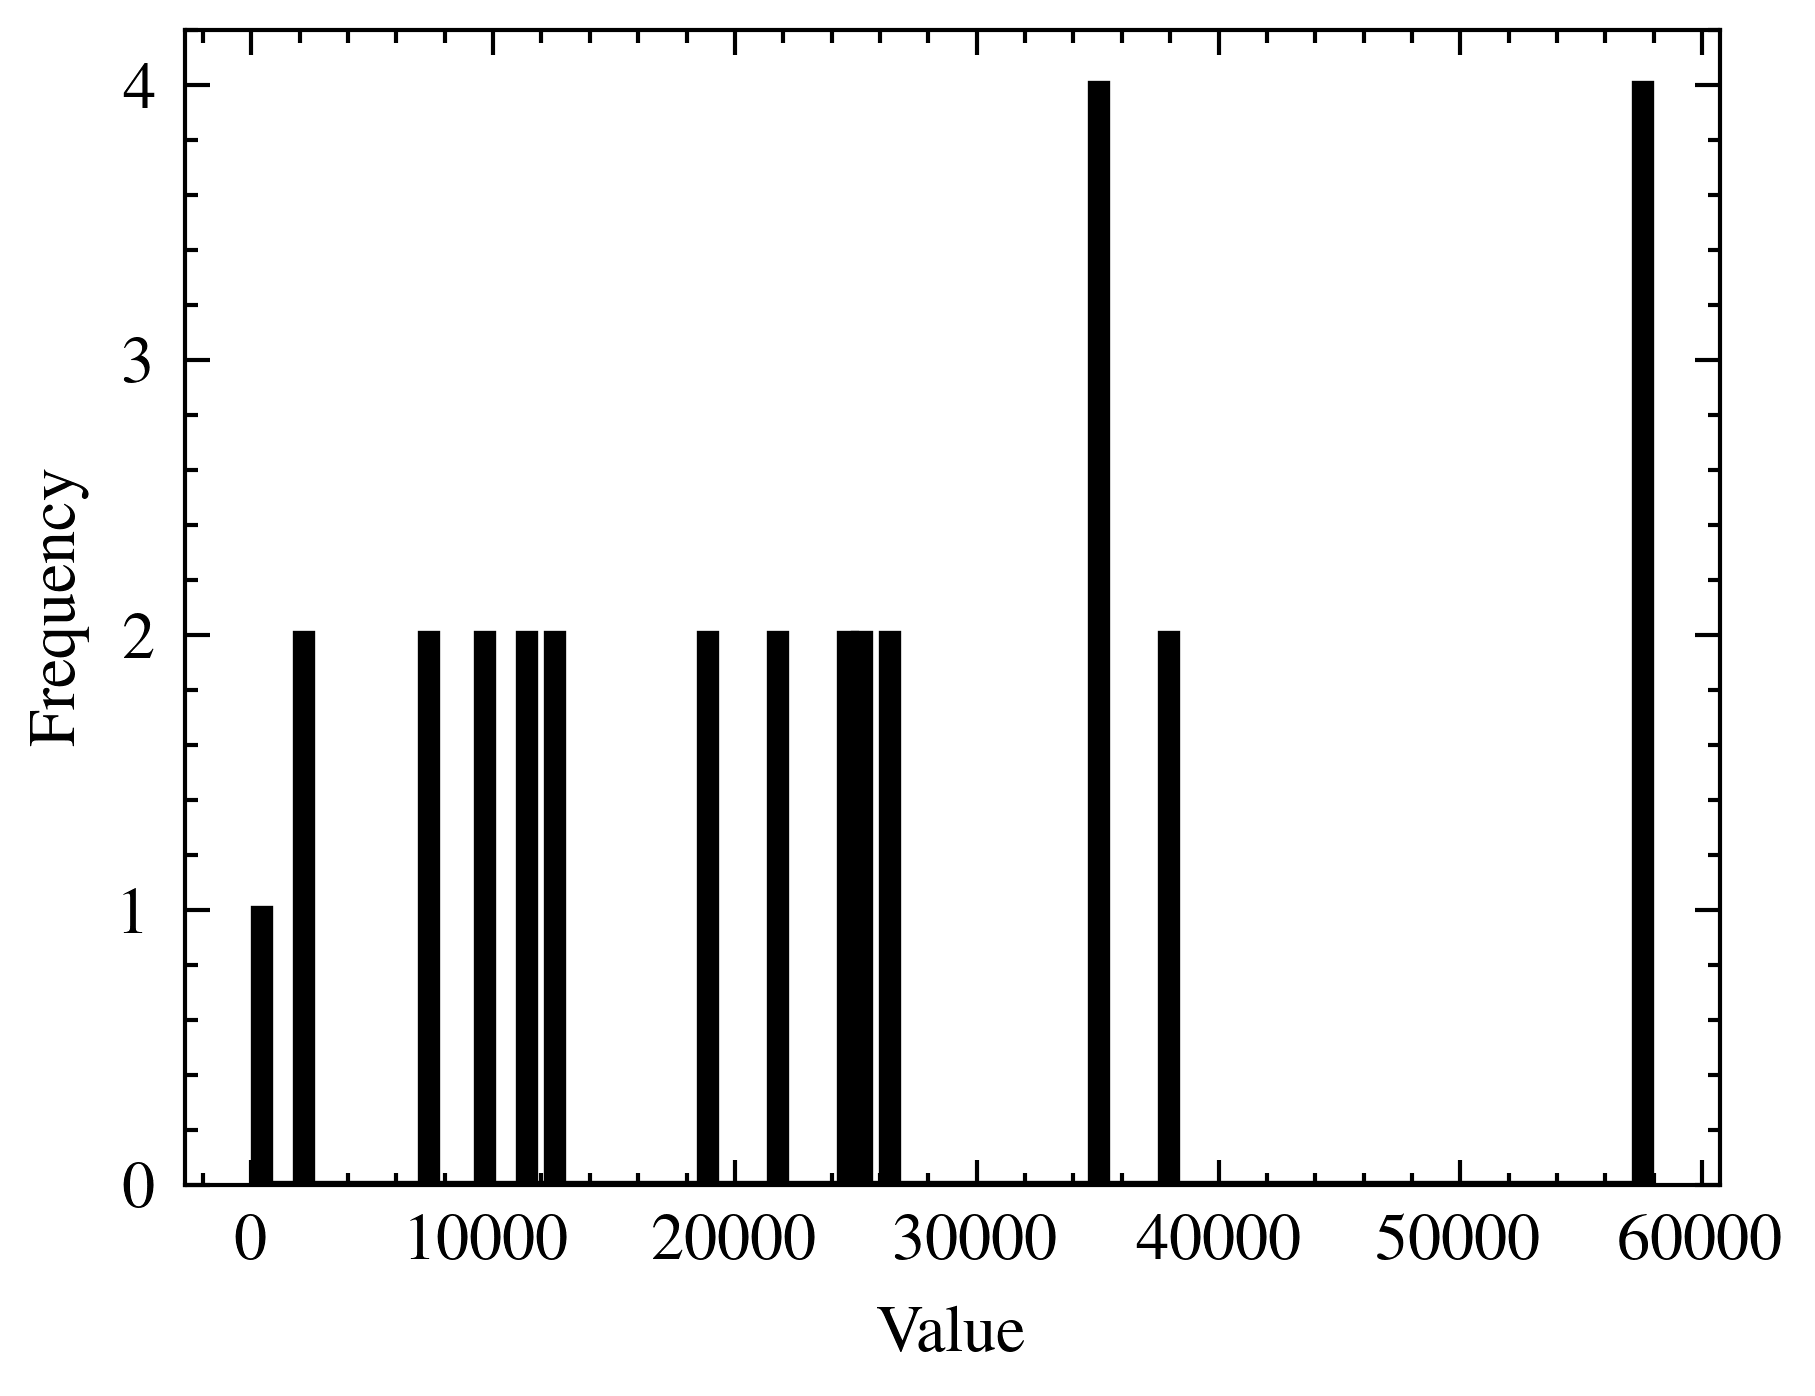
\includegraphics[width=\linewidth]{src/figures/lcg-plot/zx/lcg-2-4.png}
		\subcaption{$N=2^4$}
	\end{subfigure}
	\begin{subfigure}{0.48\linewidth}
		\centering
		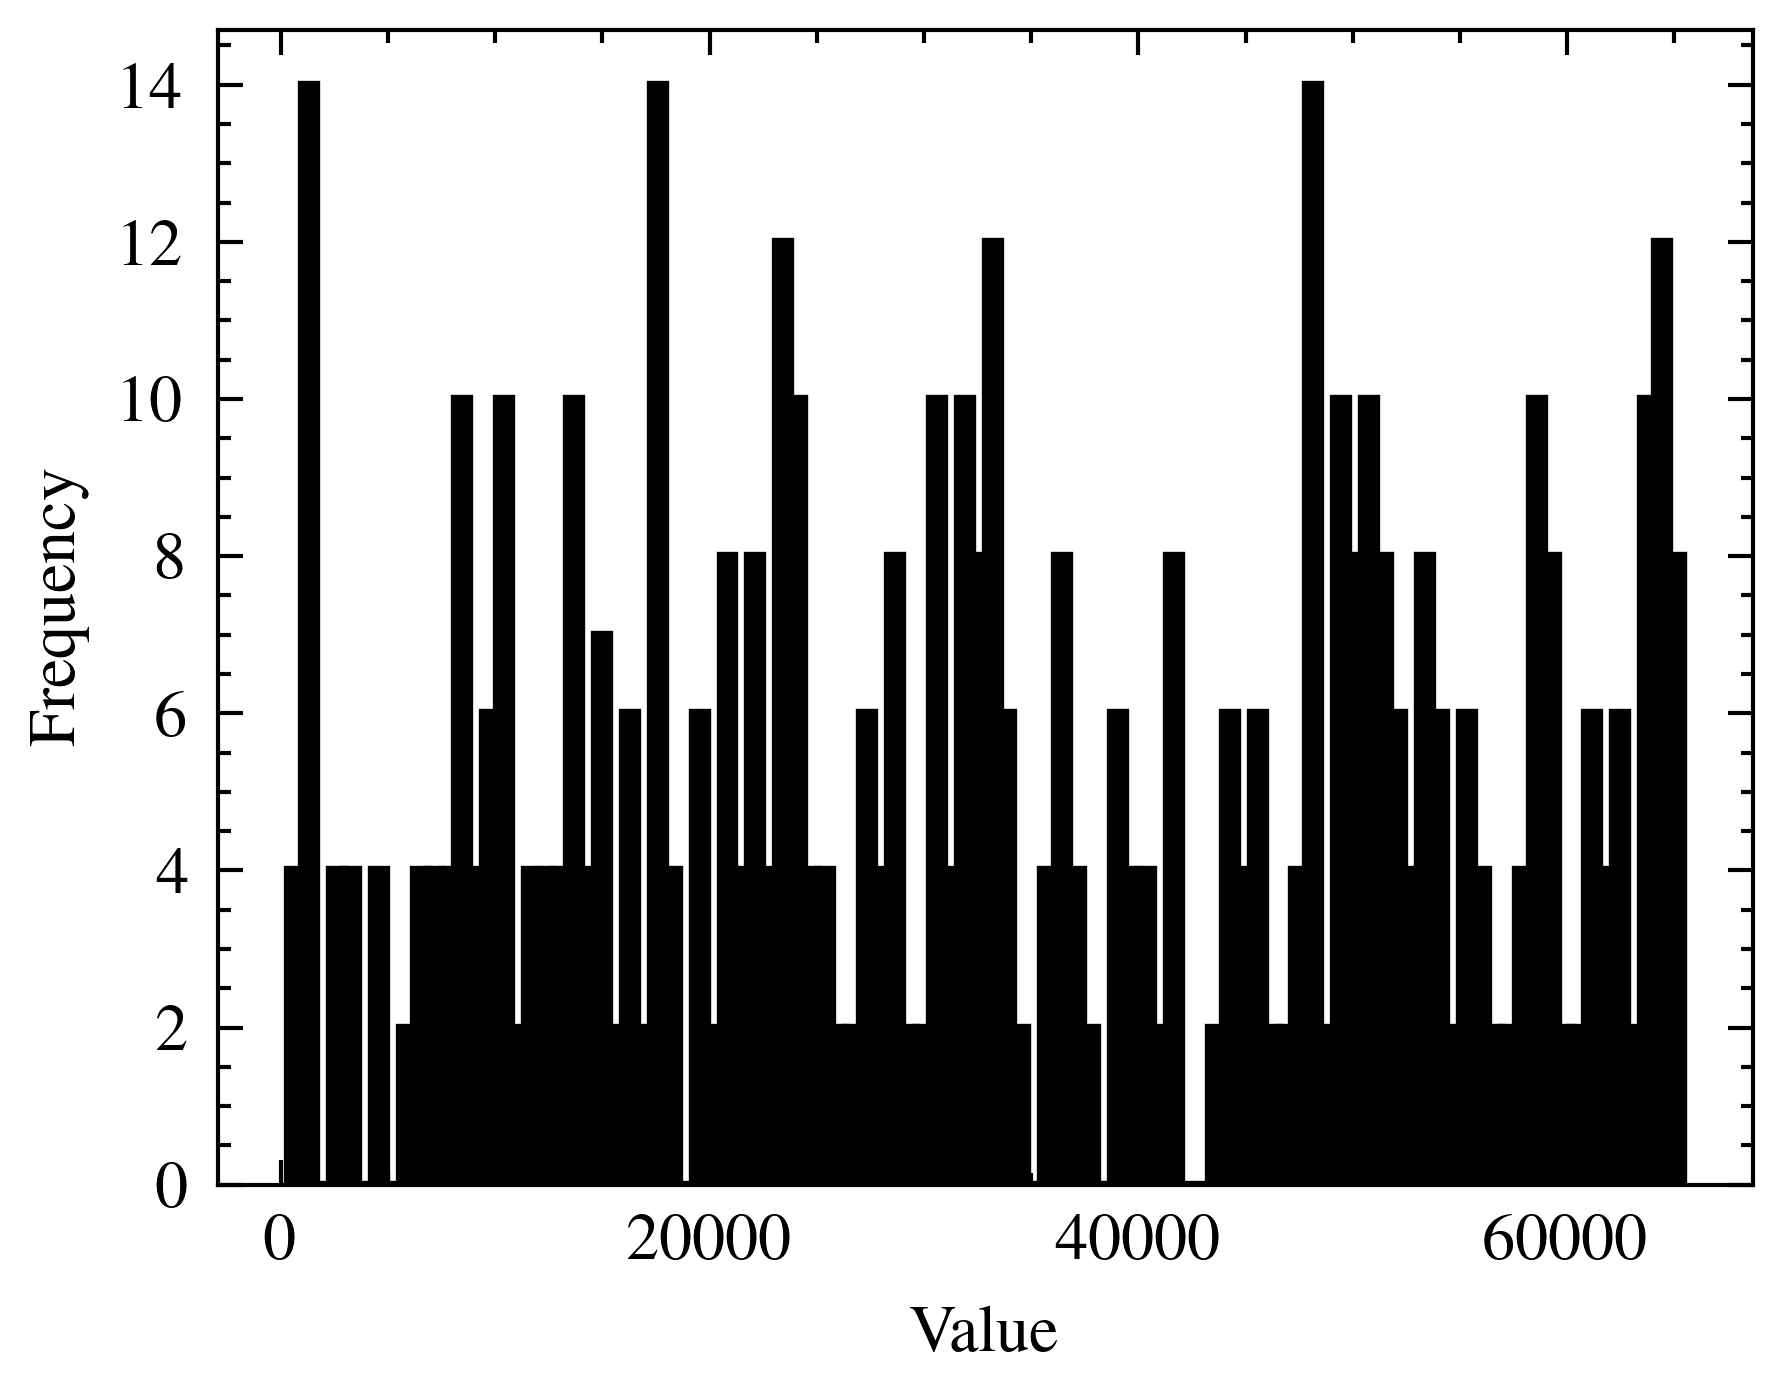
\includegraphics[width=\linewidth]{src/figures/lcg-plot/zx/lcg-2-8.png}
		\subcaption{$N=2^8$}
	\end{subfigure}
	\begin{subfigure}{0.48\linewidth}
		\centering
		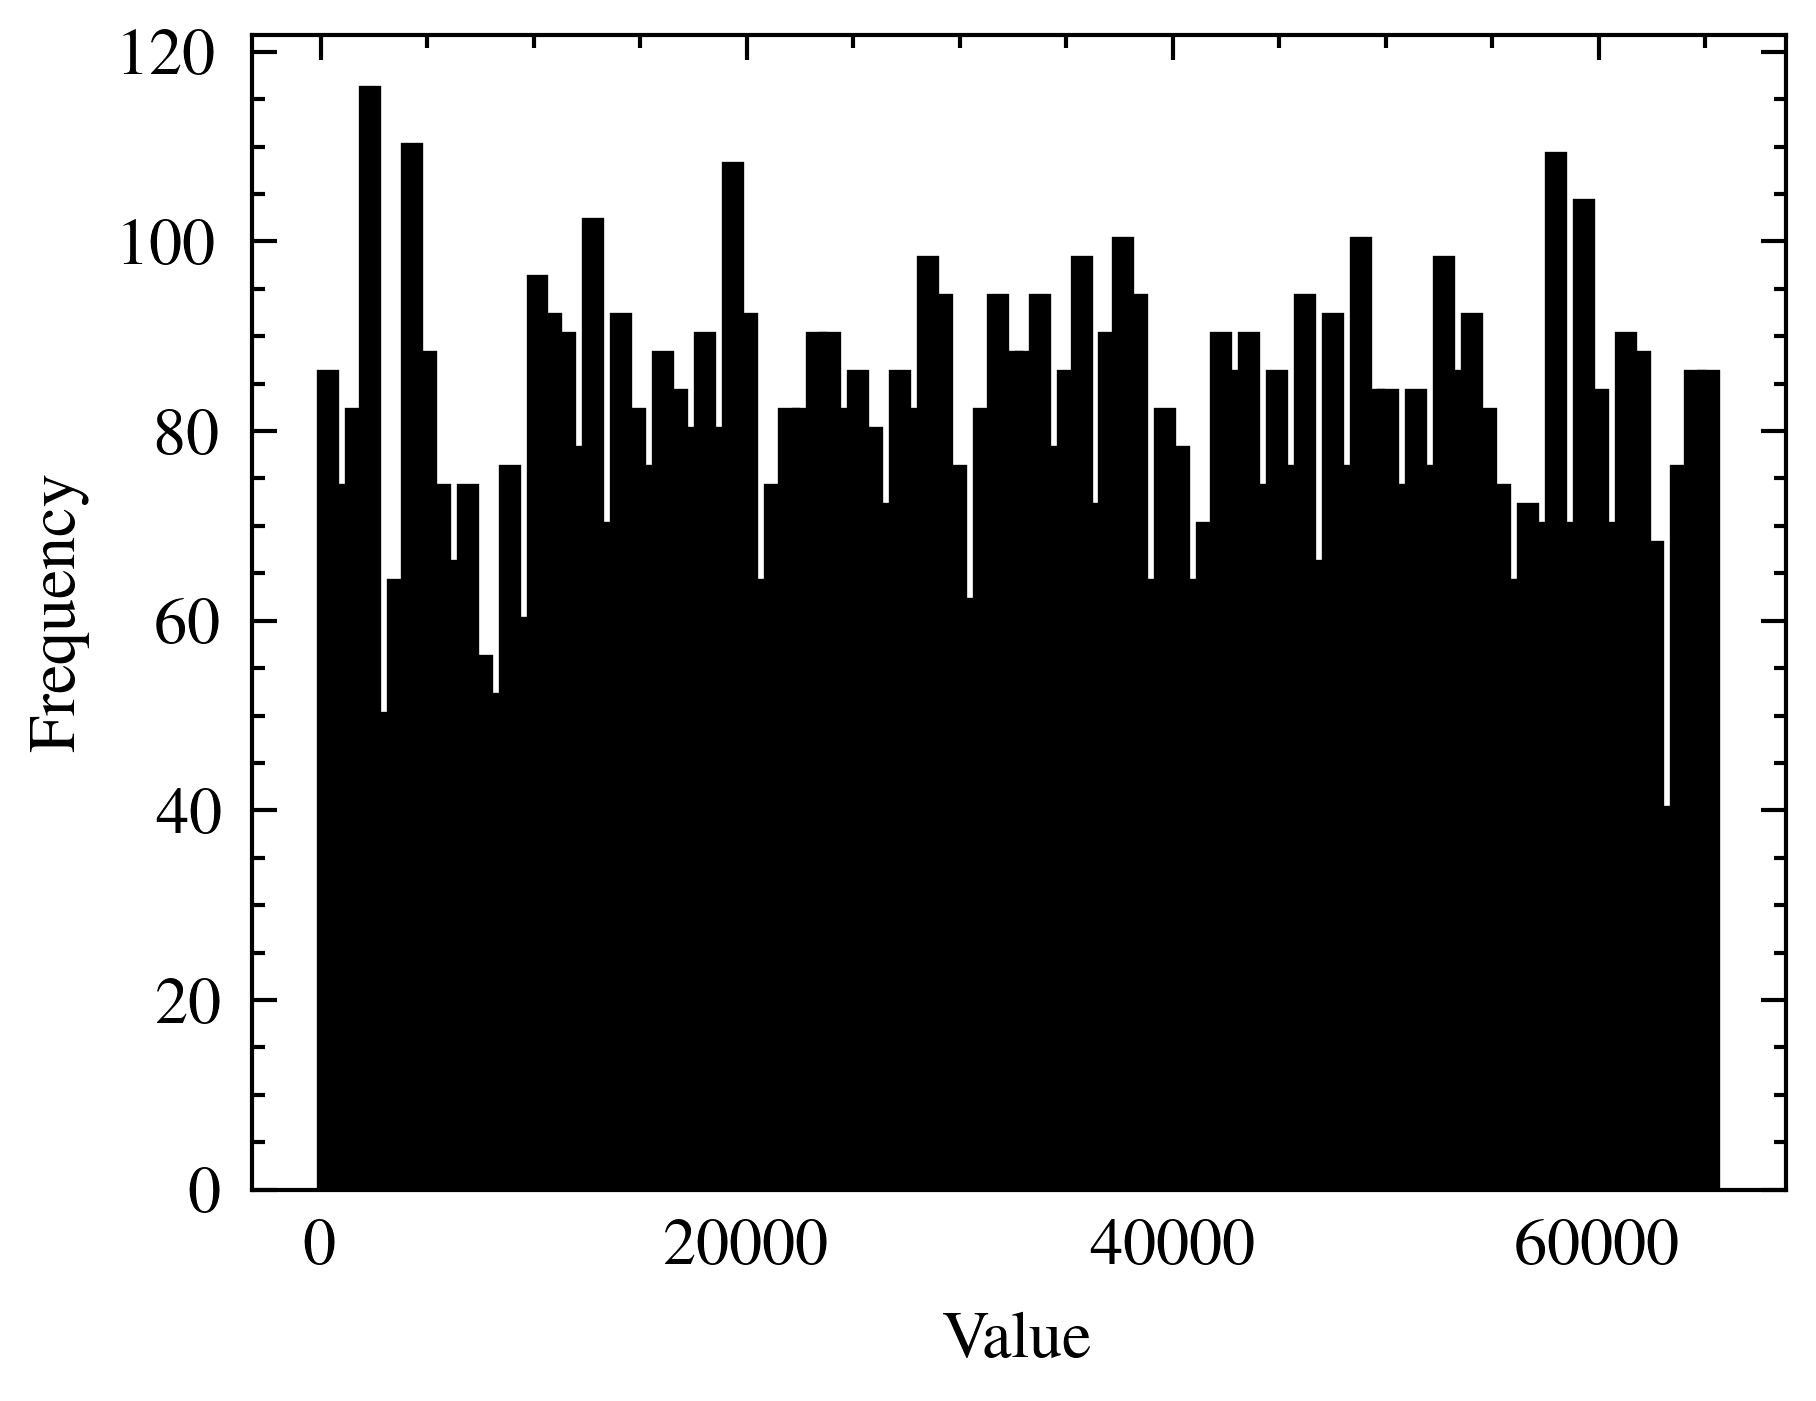
\includegraphics[width=\linewidth]{src/figures/lcg-plot/zx/lcg-2-12.png}
		\subcaption{$N=2^{12}$}
	\end{subfigure}
	\begin{subfigure}{0.48\linewidth}
		\centering
		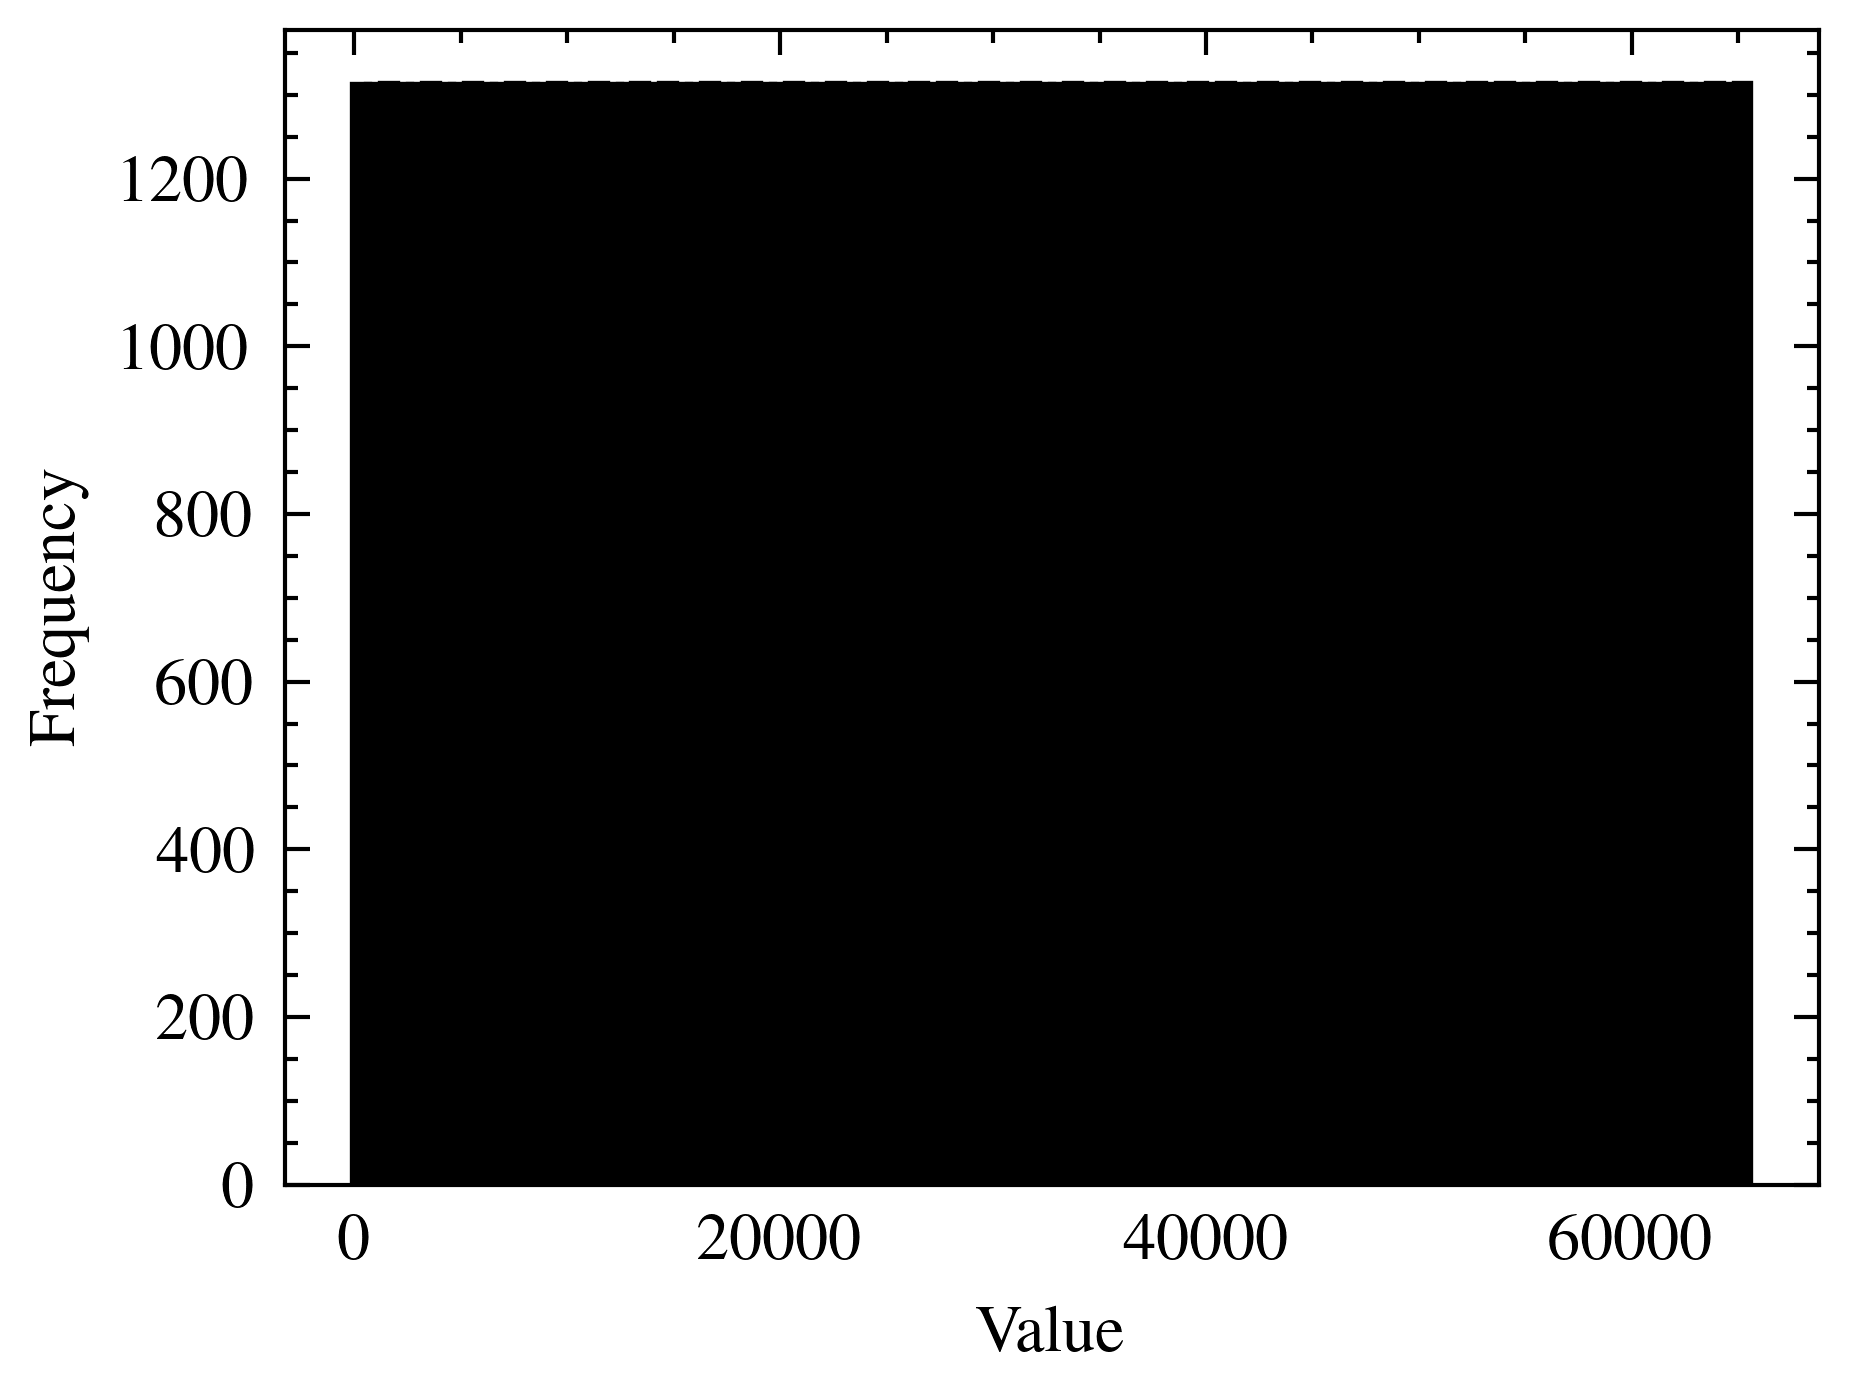
\includegraphics[width=\linewidth]{src/figures/lcg-plot/zx/lcg-2-16.png}
		\subcaption{$N=2^{16}$}
	\end{subfigure}
	\caption{線形合同法の乱数生成 $a=75, c=74, m=2^{16}+1$}\label{fig:lcg-zx}
\end{figure}

\begin{figure}
	\centering
	\begin{subfigure}{0.48\linewidth}
		\centering
		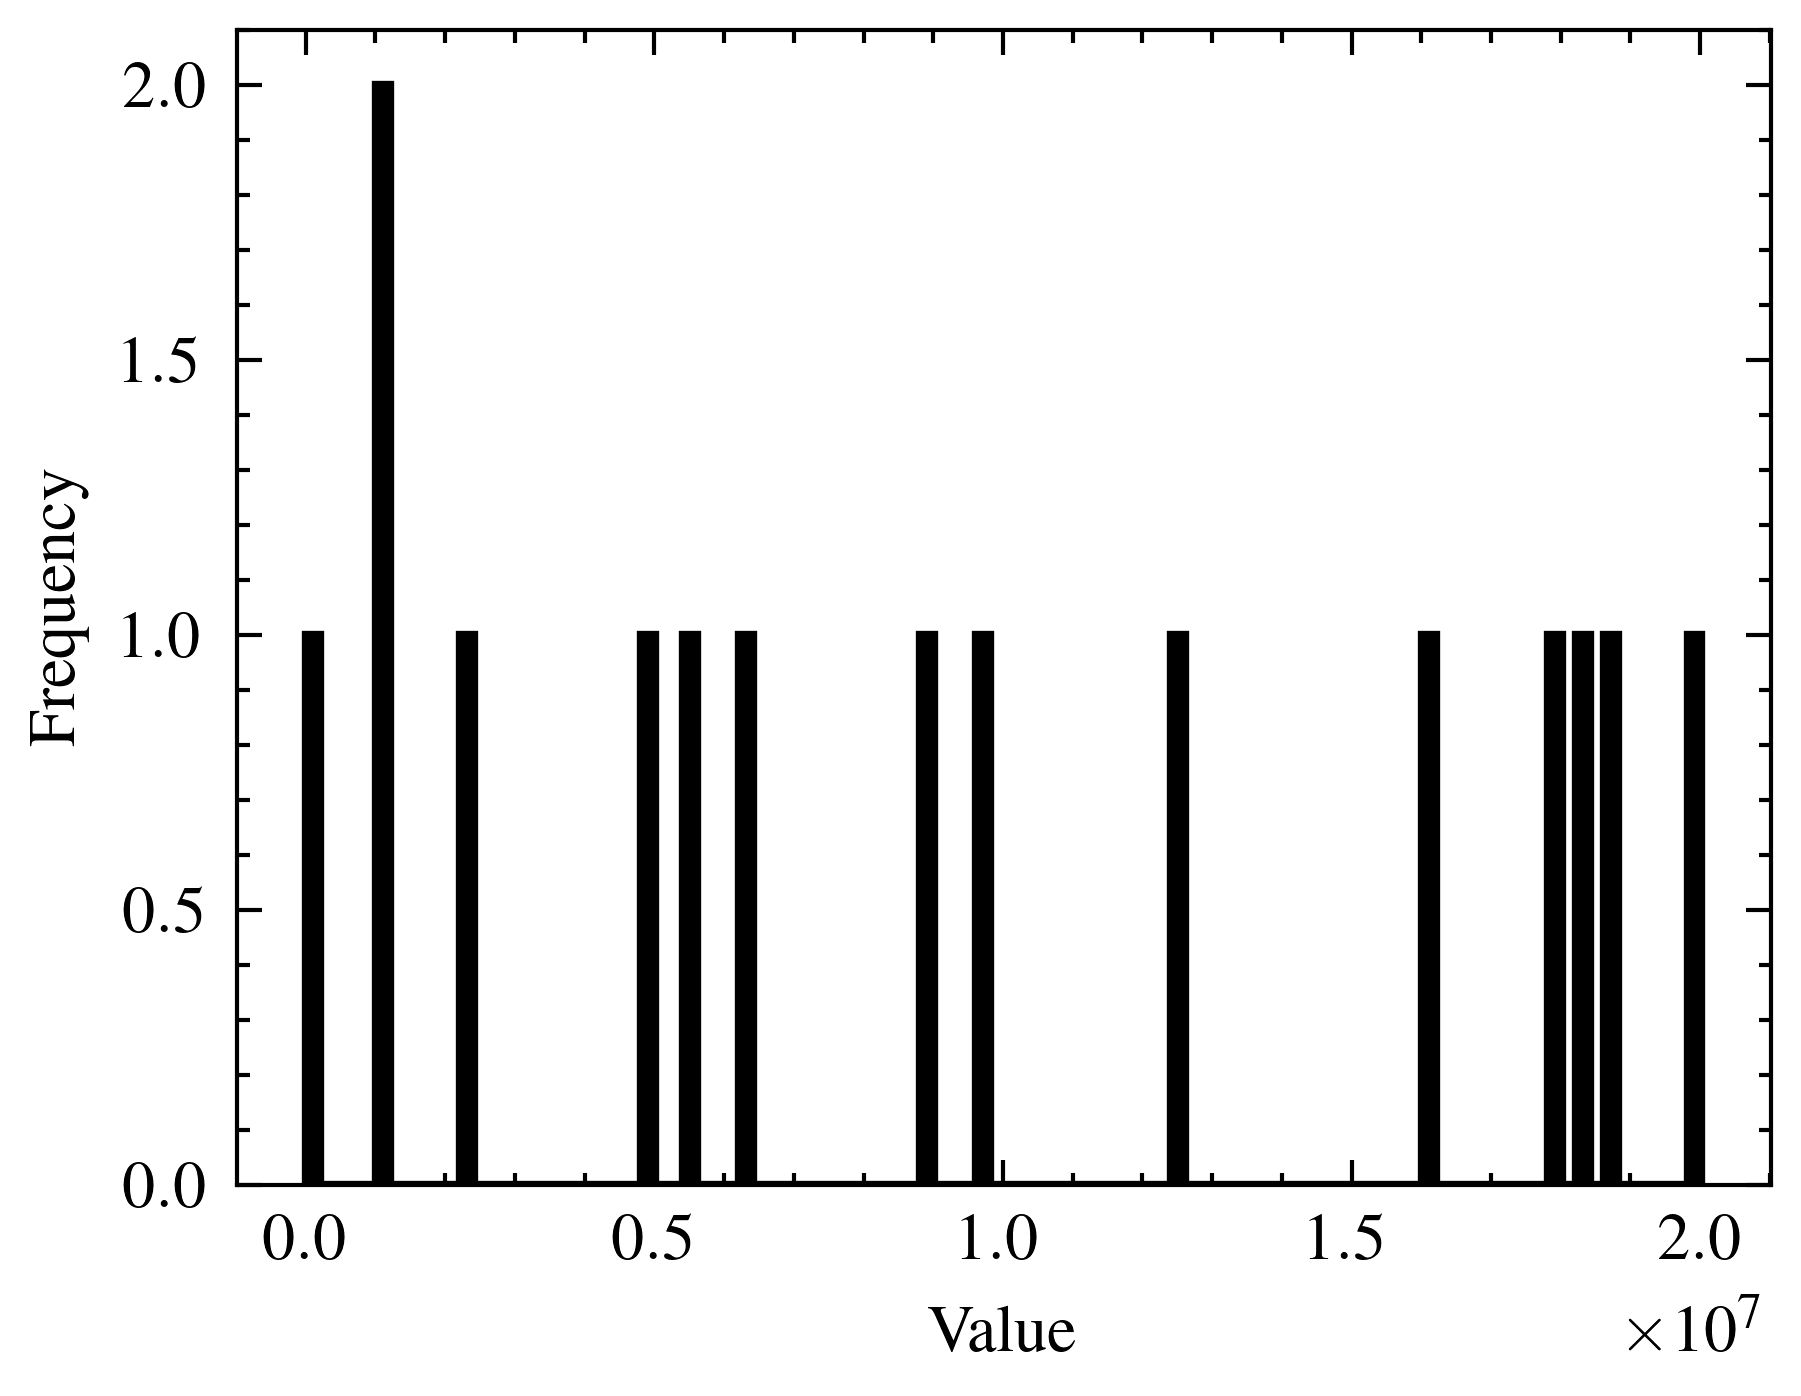
\includegraphics[width=\linewidth]{src/figures/lcg-plot/rand/lcg-2-4.png}
		\subcaption{$N=2^4$}
	\end{subfigure}
	\begin{subfigure}{0.48\linewidth}
		\centering
		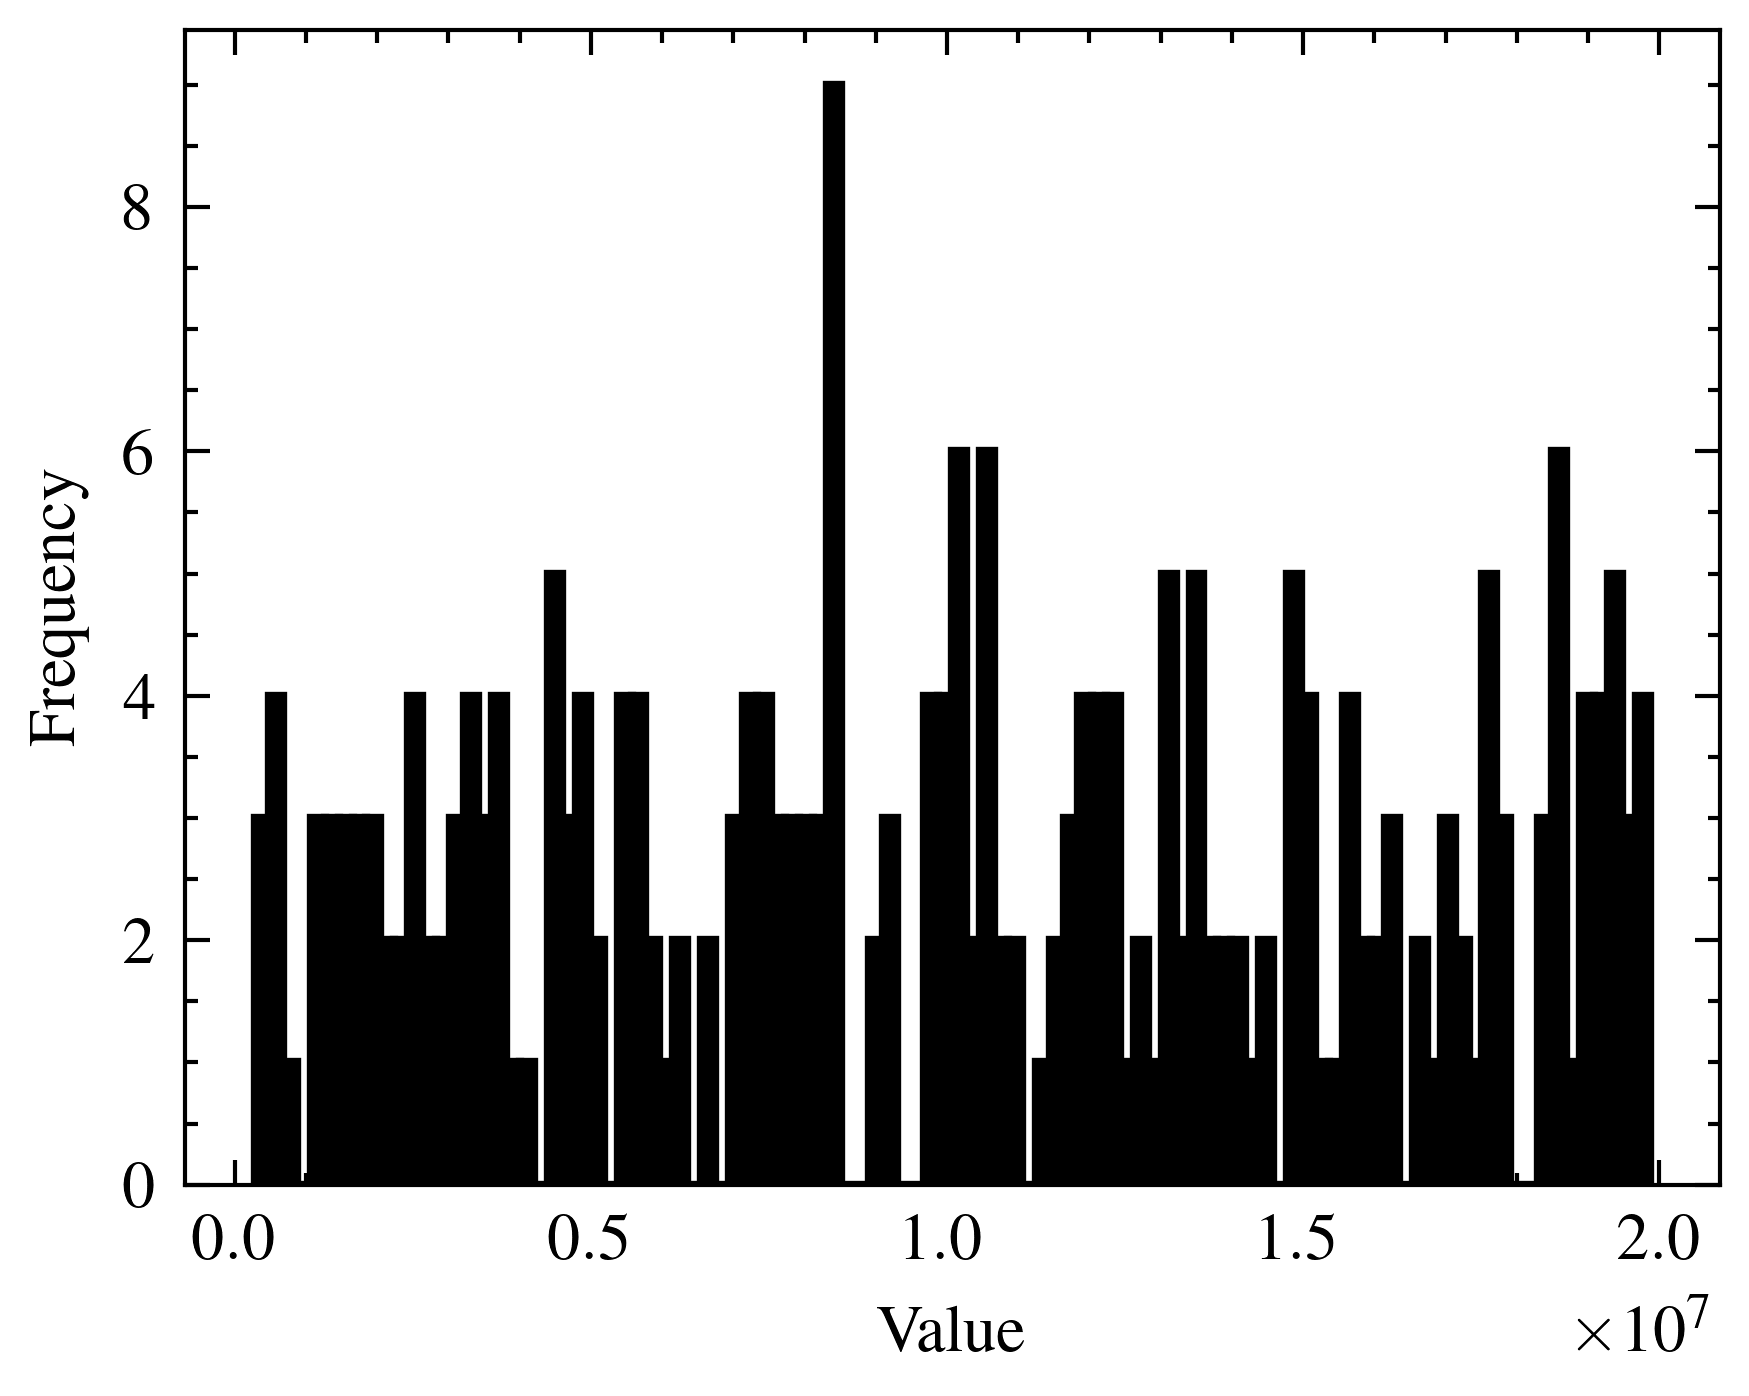
\includegraphics[width=\linewidth]{src/figures/lcg-plot/rand/lcg-2-8.png}
		\subcaption{$N=2^8$}
	\end{subfigure}
	\begin{subfigure}{0.48\linewidth}
		\centering
		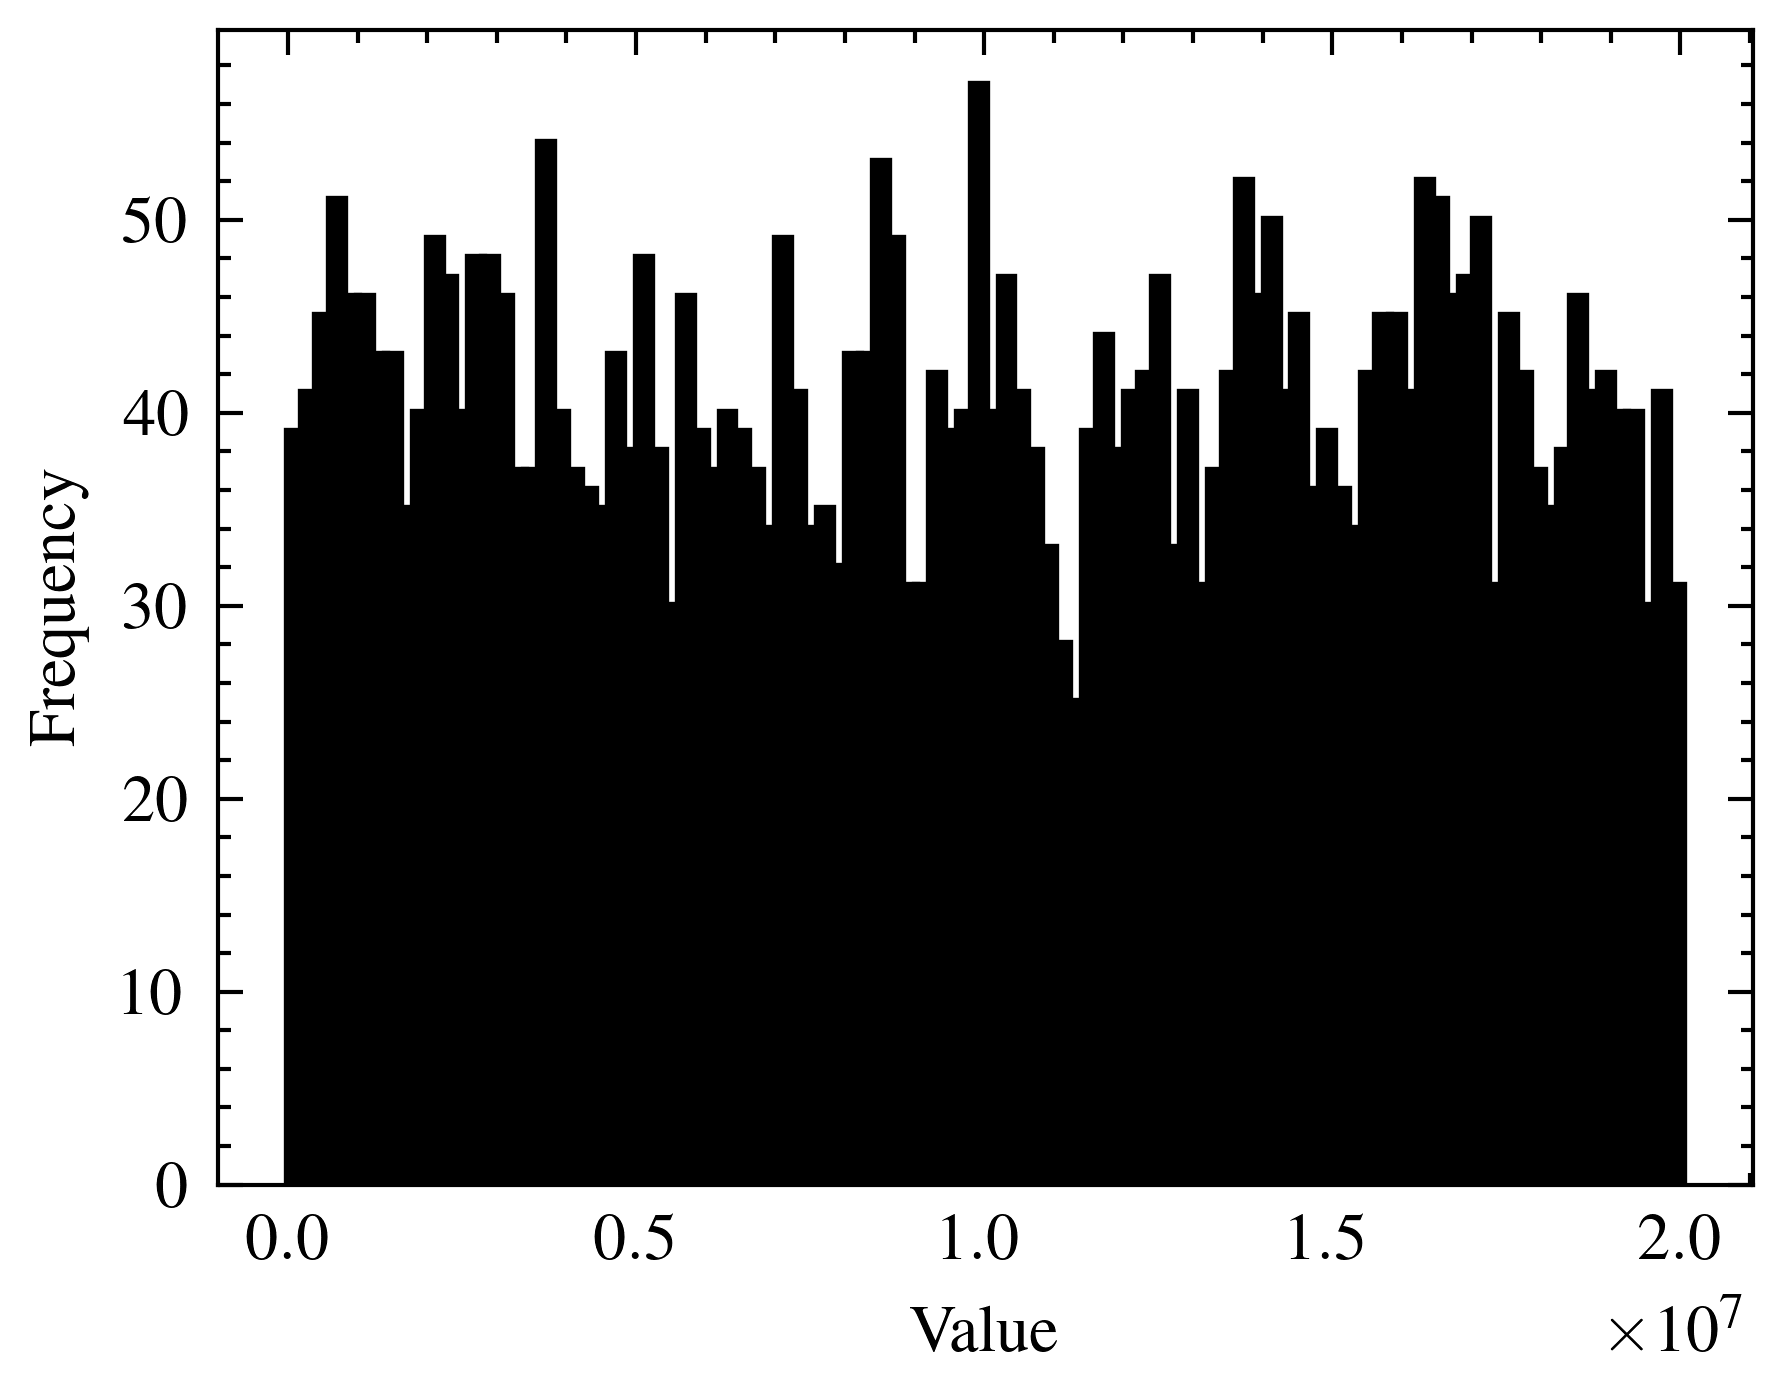
\includegraphics[width=\linewidth]{src/figures/lcg-plot/rand/lcg-2-12.png}
		\subcaption{$N=2^{12}$}
	\end{subfigure}
	\begin{subfigure}{0.48\linewidth}
		\centering
		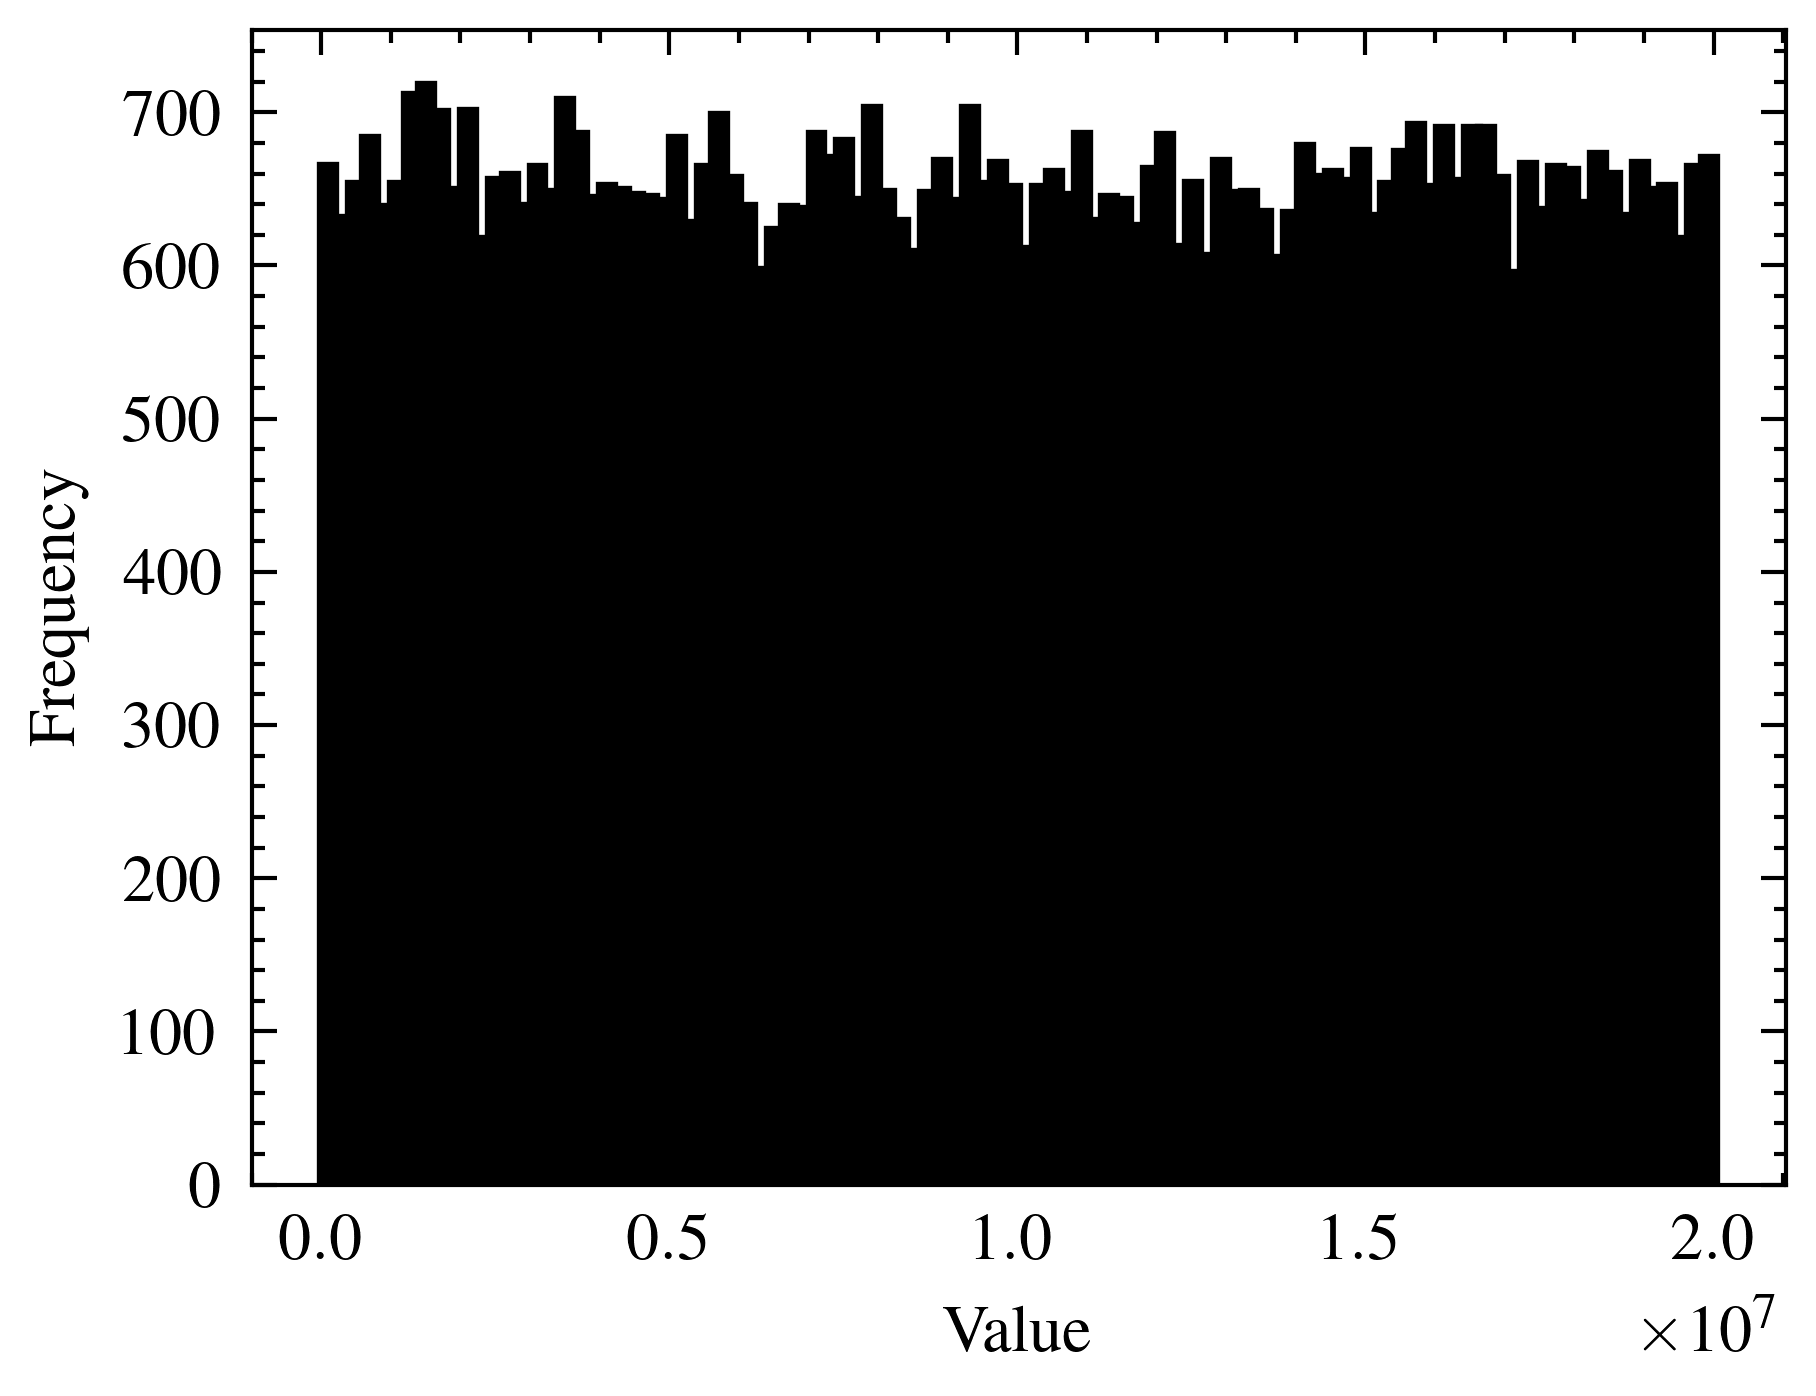
\includegraphics[width=\linewidth]{src/figures/lcg-plot/rand/lcg-2-16.png}
		\subcaption{$N=2^{16}$}
	\end{subfigure}
	\caption{線形合同法の乱数生成 $a=101, c=49, m=20040213$}\label{fig:lcg-rand}
\end{figure}
